\chapter{String Matching}

\section{Intro to biology}
DNA (Deoxyribose Nucleic Acid) is the nucleic acid which encodes the genetic program of both \textbf{prokaryotes} (bacteria and archea) and \textbf{eurkaryotes} (animals and plants). It is composed by long polymer (chains) made from repeating units called \textbf{nucleotides} or \textbf{bases}, that are \textit{adenina} (A), \textit{cytosine} (C), \textit{guanine} (G) and \textit{thymine} (T). The relation preserved inside the DNA establish that $A$ pairs with $T$ and $C$ pairs with $G$.

\begin{itemize}
	\item Adenine and guanine are purines, containing a pair of connected rings.
	\item Cytosine, thymine and uracil are pyrimidines and they are composed by a single ring.
\end{itemize}

A gene is a region of DNA that controls a hereditary characteristic, usually corresponding to a single mRNA which will be translated into a protein.

\section{Pattern matching}
This problem of pattern matching is a general task in computer science, also in biology it is an important point since it allows us to compare DNA or RNA strings.\\
Pattern matching can be defined as \textit{"Given a text T and a pattern P, determine all the occurrences of the pattern in the text"}. It is a common problem in biology since finding the exact matchings of a pattern in a biological sequence has a precise meaning in terms of evolution and functions.
First of all, it is essential to understand the way in which strings are defined during this course:
\begin{itemize}
	\item $\mathbf{S}$, it is a string of $k$ symbols, ($ 1 \leq h \leq k $).
	\item $\mathbf{S[1\dots h]}$ or $\mathbf{S_h}$, it is a prefix of $h$ symbols, ($S[1 \dots h] ~~ [ S ~~ or ~~ S_h[ S $).
	\item $\mathbf{S[h \dots k]}$, it is a suffix of $k-h+1$ symbols, ($S[h \dots k] ~~ ]S$).
	\item $\mathbf{S[i \dots j]}$, it is a substring of $j-i+1$ symbols, ($0 \leq i \leq j \leq k$).
	\item $\mathbf{S(h)}$, it is the $h$-th symbol in S.
\end{itemize}
In a more formal way, it is possible to define the pattern matching procedure as:
\par \medskip \noindent
Given $T[1 \dots n]$ and $P[1 \dots m]$, $m \leq n$, $\Sigma$ common alphabet of $T$ and $P$, we want to find all the $s$, $0 \leq s \leq n-m$, such that $T[s+1 \dots s+m] = P[1 \dots m]$.

\subsection{Pattern matching: Naive algorithm}
The algorithm can be interpreted graphically as sliding the pattern over the 
text.
\image{img/naive_algorithm}{Naive algorithm implementation.}{0.7}
\textbf{Time complexity}: $O((n-m+1)m)$ in the worst case, since the algorithm compares two strings of size $m$ for each available shift of the pattern in the text $(n-m+1)$. Considering the example in which we have $T = a^n$ and $P = a^m$, in case $m=n/2$, we've got a complexity of $O(n^2)$.\\
The problem of this solution is that we are comparing multiple time the same symbol in $T$, increasing the number of operations needed. There is no pre-processing and each time we are looking for a match we have to do it online paying the previous complexity.

\subsection{Pattern matching with FA}
The algorithm uses a \textbf{finite automaton} to solve the problem. 
\image{img/FA}{Finite automaton example.}{0.8}
A complete FA always proceeds in $T$ and no symbol is inspected more than once. It is possible to notice that the state $i$ represents the recognition of the first $i$ symbols of $P$, indeed, every state represents a prefix of $P$.\\
A finite automaton is defined as $M = (Q, q_0, A, \Sigma, \delta)$, where:
\begin{itemize}
	\item $Q$ is the finite set of states.
	\item $q_0$ is the initial state.
	\item $A$ is the set of accepting states, $A \subset Q$.
	\item $\Sigma$ is the finite input alphabet. It contains the symbols that compose the pattern.
	\item $\delta: Q \times \Sigma \rightarrow Q$ is the transition function.
\end{itemize}
$M = (Q, q_0, A, \Sigma, \delta)$ induces a function called the \textit{final state} function, $\phi: \Sigma^* \rightarrow Q$ such that $\phi(w)$ is the state $M$ ends up in after scanning the string $w$.
\par \bigskip \noindent
The \textbf{suffix function} $\sigma: \Sigma^* \rightarrow\{ 0,1, \dots, m\}$. It is possible to say that $\sigma(x)$ gives the length of the longest prefix of $P$ which is also a suffix of $x$, where $x$ indicates the already read text.
$$\sigma(x) = max\{k~|~ P[1\dots K]~~ \mathbf{\big]} x\} \qquad \sigma(x) = m \quad \text{iff  } \text{P \textbf{]} x} \quad \sigma \text{ is maximum when P is a suffix of x}$$
If $P=at$ we have that $\sigma(\varepsilon) = 0$, $\sigma(ccaca) = 1$ and $\sigma(atcat) = 2$.

\paragraph{FA Algorithm.} One of the main characteristics of FA algorithm is that it is an on-line algorithm with time complexity equal to $O(n)$. But what is missing here is the cost of the pre-processing step required to build the function $\delta$:

$$ \delta(q,a) = \sigma(P[1\dots q]a)$$
which is a map to a state representing the longest prefix of $P$ which also suffix of $P[1\dots q]a$.\\
Then, once we have computed with the pre-processing step the $\delta$ function we can define the following online algorithm for finding matches of the pattern in $T$.

\image{img/FA_algorithm}{Finite automaton algorithm.}{0.65}

From this definition we can see that the number of iterations required for finding the pattern is $n$, which is the minimum that we can have since for sure we have to read the text. Then for each iteration it computes the $\delta$ function and if the longest prefix is equal to $m$ it means that we have a match.

\paragraph{Pre-processing of the pattern} The proposed algorithm we have seen works with the assumption of having a transition $\delta$ that is able to maps to the longest prefix. The following algorithm is defined in order to compute this function, starting from the pattern, in a pre-processing step:
\image{img/delta}{Algorithm for delta computation.}{0.5}
It has a \textbf{time complexity} of $O(m^3|\Sigma|)$ in the worst case, but the optimized versions can reach $O(m|\Sigma|)$.

Pattern matching with FA but also the Knuth-Morris-Pratt Algorithm that we will see later are based on the following idea:
\begin{itemize}
	\item \textbf{Preprocessing:} process the pattern in order to determine information useful for the matching phase.
	\item \textbf{Scanning:} searching all the occurrences of  the pattern in the text. 
\end{itemize}
The complexity of these two tasks are:
\begin{itemize}
	\item Preprocessing of P: $O(m)$.
	\item Search of the pattern in $T$: $O(n)$.
\end{itemize}
Hence, an optimum pattern matching algorithm requires $O(n+m)$ in the worst case.

In this case, it is possible to highlight advantages and drawbacks.
\begin{table}[H]
	\centering
	\begin{tabular}{| p{7.5cm} | p{7.5cm} |}
		\hline
		\textbf{Pros} &  \textbf{Cons}\\
		\hline
		Efficient: it inspects any symbol in $T$ only once. & We need to build an appropriate FA.\\
		\hline
		Time complexity: $O(n)$. & Pre-processing of $P$ requires $O(m|\Sigma|)$ using an optimum algorithm.\\
		\hline
	\end{tabular}
\end{table} 

\subsection{Questions}
\begin{enumerate}
	\item \textbf{What is the advantage of pre-processing} $P$\textbf{?} The main advantage is that once we have computed the transaction function $\delta$ we are sure that it will be always the same, since depends only on the pattern, and we can use it again with other texts. The idea is that we can reuse the same function and looking for the same pattern in different sequences/text.
	\item \textbf{What could be the best use of the pre-processing?} The best that we can do is to store the automaton so that we pay only once the cost of computing it and we reduce the complexity of the algorithm only to the scanning complexity, which we have seen is $O(n)$.
	\item \textbf{If we have a finite set of patterns} $\{P_1, P_2, \dots, P_r	\}$ \textbf{to be searched in} $T$, \textbf{how can we do?} Instead of having $r$ different automaton and for each of them a scanning phase is required, we can build a unique automaton which contains all the $r$ patterns. The idea is that using multiple automaton we have to read the text $r$ each symbol of the text. However having a unique automaton we only need to scan the text only once to find the occurrences of the $r$ patterns.
\end{enumerate}

\section{Knuth-Morris-Pratt algorithm}
The main differences of KMP algorithm with respect to pattern matching with FA are that:
\begin{itemize}
	\item It avoids the computation of $\delta$ altogether. Instead of computing the entire function in the pre-processing step, it is able online to decide the destination state.
	\item It uses auxiliary \textbf{prefix function} $\pi[1, \dots, m]$ precomputed from $P$ in time $O(m)$.
	\item $\pi[1, \dots, m]$ allows $\delta$ to be computed "on the fly" as needed.
\end{itemize}
The \textbf{time complexity} of this KMP algorithm is $O(n)$.

\subsection{Prefix function $\pi$}
This prefix function is introduced in order to avoid the testing of useless shifts in the naive pattern matching algorithm and to avoid the pre-computation of $\delta$.\\
As it is possible to see in the next image, naive algorithm makes several useless comparison.
\image{img/naive_comparison}{Comparison with naive algorithm.}{0.75}
We can see that $P$ is aligned with $T$, so that $P[1, \dots, q] = T[s+1, \dots, s+q]$. Knowing these $q$ symbols we can immediately determine that some shifts are not valid ($s+1, s+2$ for example). It can be noticed also that $AG$ is both a suffix and a prefix of $P[1, \dots, q]$ and then the first valid shift is $s+3$, this means that also the comparison of $s+4$ and $s+5$ could be avoided. In other words it allows the algorithm to not compare again symbols previously checked, limiting as a consequence the number of comparison (time complexity). \\
For these reasons, prefix function $\pi$ is introduced and $\pi[q]$ can be defined as the length of the longest prefix of $P$ which is also a suffix of $P_q$. In other words it maps to the latest occurrence of a prefix of $P$.
\image{img/prefix_fun}{Prefix function $\pi$.}{0.75}

\begin{lstlisting}[escapeinside={(*}{*)}]
# Examples of computing (*$\pi$*)  
Pattern: (*\verb|a a a a a|*)
	(*$\pi$*):	    (*\verb|0 1 2 3 4|*)

Pattern: (*\verb|a b a b a b|*)
	(*$\pi$*):	    (*\verb|0 0 1 2 3 4|*)

Pattern: (*\verb|a b a c a b a b|*)
	(*$\pi$*):	    (*\verb|0 0 1 0 1 2 3 2|*)

Pattern: (*\verb|a a a b a a a a a b|*)
	(*$\pi$*):	    (*\verb|0 1 2 0 1 2 3 3 3 4|*)
\end{lstlisting}
Below it is reported the implementation of the prefix function $\pi$, in slides [25-30], it is also possible to find an example of execution of this algorithm.
\image{img/prefix_fun_algorithm}{Prefix function $\pi$ implementation.}{0.75}
\paragraph*{$\pi$ time complexity.} The overall \textbf{time complexity} of this function is $O(m)$.
\image{img/prefix_fun_complexity}{Prefix function $\pi$ implementation.}{0.75}
\subsection{KMP implementation}
By using the prefix function, it is possible to give an algorithm that reads the text $T$ symbol by symbol, without backtracking (\textit{on-line algorithm}). It doesn't read the pattern $P$ from the beginning every time, in this way overlapping parts (the longest prefix that is also a suffix) are skipped. It is a very good algorithm for texts with many repetitions.\\
In the end, the final KMP algorithm implementation can be observed in the following. Also an example of the algorithm execution can be found from slide 35 to 47.
\image{img/KMP_algorithm}{KMP algorithm implementation.}{1}

\paragraph*{KMP time complexity.} The time complexity is determined by the following elements:
\begin{itemize}
	\item \verb|ComputePrefixFunction| costs $O(m)$ as we saw before.
	\item The cycle costs $O(n)$, it is linear with respect to the text length.
	\item The instructions inside the cycle have a constant time.
\end{itemize}
Hence, the time complexity of KMP algorithm is $O(m+n)$. In order to give a better idea of the complexity of this algorithm we have used the \textbf{amortized analysis}, which is different from average case analysis in that the probability is not involved. An amortized analysis guarantees an average performance of each operation in the worst case.

\subsection{Summary}
\begin{itemize}
	\item Computing the $\pi$ table is independent of the text string to search. So if the same pattern is used on multiple texts, the table can be pre.computed and reused. The KMP algorithm always requires $O(m)$ extra space for the $\pi$ table.
	
	\item If pre-computation is performed, then preprocessing the pattern takes $O(m)$ time and searching the text takes worst-case $O(n)$ time (instead of the combined $O(m + n)$ time stated at the beginning of the article).
	
	\item The text string can be streamed in because the KMP algorithm does not backtrack in the text. This is another improvement over the naive algorithm, which doesn’t naturally support streaming. If streaming, the amortized time to process an incoming character is $O(1)$ but the worst-case time is $O(min(m, n^\prime))$, where $n^\prime$ is the number of text characters seen so far.	
\end{itemize}


\newpage

\section{Suffix Trees}
A suffix tree is a data structure able to represent a string and its “internal structure”. It is used for pattern matching but also for other strings problems, in pattern matching it is used to do the preprocessing of $T$ (instead of $P$), that allows to search many patterns in the same text.

\subsection{Suffix tree definition} 
Let $S$ be a string with $n$ symbols:
\begin{enumerate}
	\item A suffix tree $\mathcal{T}$ for $S$ is a (directed) tree with $n$ leaves, numbered from 1
	to $n$, one for each suffix of $S$.
	\item Each internal node has at least $2$ sons and any arc is labeled with a 
	nontrivial substring of $S$.
	\item Outgoing arcs from a node are labeled with different initial symbols.
	\item For any leaf $i$, the concatenation of the labels of the arcs, in the path from the root to $i$, is $S[i \dots n]$.
\end{enumerate}
\image{img/suffix_tree_example}{Suffix tree example.}{0.6}
The suffix tree may not exist for some $S$ if a suffix $s$ of $S$ is a prefix of another suffix $r$ of $S$ (Ex: $S = xabxa$, $s=xa$, $r=xabxa$). For this reason, a new symbol \$ is added at the bottom of $S$.
\image{img/hattivatti}{Example of suffix tree with \$.}{0.6}
\newpage
After this quick introduction it is possible to notice some definitions related to suffix trees:
\begin{itemize}
	\item \textbf{Label of a path}: concatenation of the strings labelling the arcs in the path.
	\item \textbf{Label of a node $v$}: label of the path from the root to $v$.
	\item \textbf{String depth of a node $v$}: number of symbols in the label of $v$. 
\end{itemize}
Suffix trees also enjoy the property that a suffix tree representing a text $T$ of length $n$ has:
\begin{itemize}
	\item A maximum number of nodes equal to $2n - 1$.
	\item A maximum number of edges equal to $2(n-1)$.
\end{itemize}
\subsection{Pattern matching by suffix tree}
Starting from the idea that given a text $T$, every substring $S$ of $T$ is the prefix of a suffix, the construction of a suffix tree for the text $T$ is very useful because $S$ can be found in our suffix tree by going through a unique path starting from the root.\\
The building of a suffix tree $\mathcal{T}$ for $T$ is made in $O(n)$ through the \textbf{Ukkonen algorithm}. In order to find all the occurrences of $P$ in the text $T$, a match of $P$ along a unique path in $\mathcal{T}$ is done until $P$ is complete or a mismatch is reached. In the first case, any leaf of the subtree rooted in the node after the last match corresponds to the position of an occurrence of $P$ in $T$, instead in the second case, $P$ doesn't occur in $T$.\\
The time complexity for this structure is composed by two different aspects:
\begin{itemize}
	\item \textbf{Preprocessing step}: $O(n)$.
	\item \textbf{Searching step}: it can be divided in $O(m)$ for traversing the path (since the alphabet is finite) and in $O(k)$ for traversing the subtree, where $k$ is the number of occurrences of $P$ in $T$. For this step, so, the final complexity is $O(m+k)$.
\end{itemize}
The overall time complexity for a pattern matching in a suffix tree is $O(n+m+k)$. 

\subsection{Naive algorithm}
This method allows us to build the suffix tree for $S[1, \dots, n]$ in $O(n^2)$. The construction of this tree can be formalized as follows:
\begin{itemize}
	\item The first node is the root.
	\item The first arc (suffix) is built with label $S[1 \dots n]\$$ and the leaf is labeled with 1.
	\item For $i$ from 2 to $n$, the added paths are labeled by the suffixes $S[i \dots n]\$$ and they are labeled with the corresponding leaves. 
\end{itemize}
This algorithm is \textbf{not on-line}.

\subsection{Ukkonen algorithm}
At the beginning \textbf{Ukkonen algorithm} considers an on-line algorithm which is simple but also inefficient $O(n^3)$, then we optimize it to make it linear. The algorithm builds a sequence of \textit{implicit suffix trees} for the prefixes of $S$, such that $\mathcal{T}_1$ for $S[1 \dots 1]$, $\mathcal{T}_2$ for $S[1 \dots 2]$, $\dots$, $\mathcal{T}_n$ for $S[1 \dots n]$. The last one tree $\mathcal{T}_n$ is then transformed into the suffix tree $\mathcal{T}$ for $S$.
\par \bigskip \noindent
An \textit{implicit suffix tree} for $S$ is the tree obtained from the suffix tree for $S\$$ by:
\begin{itemize}
	\item Removing all the occurrences of \$ from the labels.
	\item Removing all the arcs without a label.
	\item Removing all the nodes which don't have at least two sons.
\end{itemize} 
The \textit{implicit suffix tree} for $S$ has less leaves than the suffix tree for $S$ if and only if at least a suffix of $S$ is prefix of another suffix.
\par \bigskip \noindent
After having built $\mathcal{T}_1$ that is the initial step, the other trees are built.
\image{img/abstract_algorithm}{Abstract on-line algorithm.}{0.7}

In other words the algorithm can be summarized as follow:
\begin{enumerate}
	\item For each symbol of the text (\verb|for i = 1 to n-1|).
	\item Extend the implicit suffix tree from $\mathcal{T}_i$ to $\mathcal{T}_{i+1}$, applying the three rules.
	\item Search the end of the path corresponding to the suffix $S[j,i]$ of the sub-string $S[1, i]$ for which $\mathcal{T}_i$ is the implicit suffix tree.
	\item If it is necessary extends the path including the symbol $S[i+1]$ such that the suffix $S[j, i+1]$ is in the tree.
\end{enumerate}


Let $\beta = S[j \dots i]$ in extension $j$, the path with label $\beta$ is extended into one with label $\beta S(i+1)$ with one of the following rules:
\begin{enumerate}
	\item \textbf{Extend the label:} if $\beta$ ends with a leaf, $S(i+1)$ is added to the label in the last arc of the path.
	\item \textbf{Create a new branch:} if no path in the end of $\beta$ begins with $S(i+1)$, but there's at least one labeled path following $\beta$, a new leaf is created with number $j$ and the arc from $\beta$ to the leaf is labeled with $S(i+1)$. If $\beta$ terminates inside an arc, also the father node for the new leaf is created.
	\item \textbf{Do nothing:} if there's a path from the end of $\beta$ which starts with $S(i+1)$, don't do anything, $\beta S(i+1)$ is already present in the tree.
\end{enumerate}

\paragraph*{Time complexity.} After the search of the end of $\beta$, a constant time is necessary to have $\beta S(i+1)$ in the tree (application of extension $j$ with rules (1,2,3)). If the search of the end of $\beta$ is done naively (for instance searching from the root), the tree $\mathcal{T}_{i+1}$ is built from $\mathcal{T}_i$ in $O(i^2)$.\\
Finally we will have that $\mathbf{\mathcal{T}_n}$ \textbf{is built in} $\mathbf{O(n^3)}$. So why we should use \textit{Ukkonen} algorithm instead of the straightforward one that has $O(n^2)$?\\
The reason of this choice is the fact that the time complexity of $O(n^3)$ can be reduced to $O(n)$ with a few observations and implementation tricks.

\paragraph*{Suffix links.} They give the most important contribution in the acceleration of the \textit{Ukkonen} algorithm. A suffix link $(v, s(v))$ is a link from $v$ to $s(v)$. They can also be defined with the help of two different properties:
\begin{enumerate}
	\item In any implicit suffix tree $\mathcal{T}_i$, if the internal node $v$ has path-label $a \alpha$, then there's a node $s(v)$ in $\mathcal{T}_i$ with label $\alpha$. If $\alpha = \varepsilon$, the suffix link goes from $v$ to the root.
	\item In \textit{Ukkonen} algorithm, any newly created internal node will have a suffix link from it by the end of the next extension. In other words, in any phase $i+1$, if $v$ is created while performing the $j$-th extension (to insert the suffix $S[j \dots i]S[i+1]$) then $s(v)$ is necessarily created while performing the $(j+1)$-th extension (to insert the suffix $S[j+1 \dots i]S[i+1]$). If rule 2 is applied at the $j$-th extension then in $j+1$-th extension a suffix link will be created.
\end{enumerate} 
The use of suffix links is clearly an improvement over walking from the root in each extension since they provide a short cut to find end of the path. However, their usage don't improve the worst case running time.

\paragraph*{Skip/Count.} With the introduction of this further trick, it will be possible to reduce the worst case time to $O(n^2)$. The Skip/count optimization is based on the idea that starting from the previous algorithm implementation, after following the suffix link, it is possible to go down along the path with label $\gamma$ in $O(|\gamma|)$. 

\image{img/skip_count_algorithm}{Skip/count optimization trick algorithm.}{0.65}
When walking down from node $s(v)$ to leaf, instead of matching path character by character as we travel, we can directly skip to the next node if number of characters on the edge is less than the number of characters we need to travel. If number of characters on the edge is more than the number of characters we need to travel, we directly skip to the last character on that edge.
If implementation is such a way that number of characters on any edge, character at a given position in string S should be obtained in constant time, then skip/count trick will do the walk down in proportional to the number of nodes on it rather than the number of characters on it.


\image{img/skip_count_tree}{Skip/count execution.}{0.65}

An interesting useful property is the fact that for any suffix link $(v, s(v))$, the node-depth of $v$ is at most one greater than the node-depth of $s(v)$.\\
By using  skip/count, any phase of 
\textit{Ukkonen} algorithm requires time $O(n)$, indeed, in any phase $i$ there are $i+1$ extensions with $i+1 \leq n$.\\
For a better understanding, it is possible to sum up any extension as:
\begin{itemize}
	\item It goes up at most one arc, in order to find a suffix link (\textit{depth of the current node-1}).
	\item It traverses the suffix link (\textit{depth of the current node at most-1}).
	\item It follows down some nodes (\textit{+k}).
	\item It applies the extension and it may add a suffix link.
\end{itemize}
Any such operation requires a constant time, up to the down walking, hence, complexity depends on the number of traversed nodes.\\
Through the using of suffix links and skip/count, \textit{Ukkonen} algorithm requires time $O(n^2)$. Even if the time complexity has been reduced, the simple naive algorithm is still preferable.\\
A suffix tree may require $O(n^2)$ space for example when $S=abc \dots xyz$, there are 26 different edges out of the root. It is possible to understand so that the time for the algorithm is at least as large as the size of its output, so the $O(n)$ seems to be impossible.

\paragraph*{Edge-labels compression.} As said before, the space necessary for representing a suffix tree is $O(n^2)$, to reduce time complexity, it is necessary to reduce the required space, otherwise the time to traverse the tree must be at least quadratic.\\
In order to reduce the space needed, instead of using substrings for labeling, it is possible to use pair of indexes, for example $S[i \dots j]$ becomes $(i,j)$. 
\image{img/edge_labels_compression}{Edge labels compression example.}{0.95}
Through this coding only two numbers are written on each edge with a number of edges at most of $2(n-1)$. We can conclude so that a suffix tree with this representation requires only $O(n)$ space.

\paragraph*{Further optimizazions.} It is possible to observe other two further optimizations related to the third and the first rule.\\
\begin{itemize}
	\item \textbf{Rule 3}: in any phase, if extension $j$ applies \textit{rule 3}, the same rule will be applied in the next extensions, till the end of the phase (from $j+
	1$ to $i+1$). We can understand that any phase terminates as soon as \textit{rule 3} is applied for the first time, because there's no more work to be done.
	\item \textbf{Rule 1}: when a leaf is created and labelled $j$, it will remain a leaf in all successive trees created during the algorithm. For this reason, \textit{rule 1} will be always applied to extension $j$ in the next phases. For example, leaf 1 is created in the first phase, in the next phases there's a sequence of extensions with rule 1.\\
	A trick that we could apply in this case is the fact that in phase $i$, when a leaf is first created and the arc would be normally labeled with $S[p \dots i]$, instead of writing $(p \dots i)$ on the edge, we write $(p \dots e)$, where $e$ is the end of the string.\\
	
	In other words the idea is that we put in the branches the compressed labels, and instead of putting $(p,i)$, where $p$ is the starting position of the suffix and $i$ the current position, we put directly $(p,e)$ so that all the rules $1$ are applied simply increasing the value of $e$. As a consequence of this improvement all the rule $1$ operations are performed in constant time.
	\image{img/rule1Opt.png}{Rule 1 optimization.}{0.3}
\end{itemize}
Following these tricks it is possible to modify the $i+1$ phase, as it can be seen in the following image.
\image{img/phase_i+1}{Phase i+1 modified.}{0.7}

$j^*$ is the last explicit extension in phase $i+1$ and the first one in phase $i+2$.

\paragraph*{Ukkonen algorithm: overall complexity.} By using suffix links, skip/count and optimizations concerning the extension rules \verb|1| and \verb|3|, Ukkonen algorithm requires time $\mathbf{O(n)}$ to build $\mathcal{T}_1 \dots \mathcal{T}_n$.\\
$\mathcal{T}_n$ is transformed into the suffix tree for $S$ in time $\mathbf{O(n)}$. The new symbol \$ is added and another phase of Ukkonen algorithm is performed in order to build $\mathcal{T}_{n+1}$, this again requires an $\mathbf{O(n)}$ time. 

\subsection{Questions - Motifs of string $T$}
\begin{enumerate}
	\item What are the frequently occurring substrings of $T$?
	\item Longest substring that occurs at least $q$ times? 
\end{enumerate}

\image{img/motifs}{Motifs of "Hattivatti".}{0.6}

\section{Generalized Suffix Trees and Suffix Arrays}
A suffix tree can be used to represent all the substrings in a set of strings $T_1, \dots, T_k$. In this case it is possible to build a generalized suffix tree for $T_1, \dots, T_k$ in linear time, with respect to the strings total size, instead of maintaining $k$ suffix trees.
The complexity of this procedure can be indicated: $O(\sum_{i = 1,k}n_i)$, where $|T_i| = n_i$.\\
\textbf{Why we should use a generalized suffix tree?} The answer is that it can be useful and allows to look for common substrings, palindromes in a text $(T_1 = T$ and $T_2 = T_R)$, and also for text comparison.

\subsection{Generalized Suffix Tree construction}
The generalized suffix tree is constructed applying the following steps:
\begin{itemize}
	\item Concatenate the strings $T_1,\dots,T_k$ in a unique text $T = T_1~ \$_1 ~T_2 ~\$_2 ~\dots ~T_k~\$_k$, with distinct separators $\$_1 ~ \$_2 ~\dots ~\$_k$.
	
	\item Apply Ukkonen algorithm to build the suffix tree for $T$, $O(\sum_{i = 1,k}n_i)$.
	
	\item Traverse the suffix tree in order to:
	\begin{itemize}
		\item Crop the string which do not belong to one single text;
		\item Annotate correctly the leaves with pairs of indexed $(i,j)$, where $i$ is the index of the text $T_i$ to which the $j$-th suffix belongs;
	\end{itemize}
\end{itemize} 
Then the overall complexity of these steps is $O(\sum_{i = 1,k}n_i)$.\\

\image{img/generalizedSuffixTree.png}{Generalized Suffix Tree construction mt1}{0.6}
The algorithm just proposed is considered as a first method, but there is another one for building the generic suffix tree:

\begin{itemize}
	\item Apply Ukkonen algorithm to build the suffix tree for $T_i\$_i$ $ \rightarrow O(n_i)$
	\item Repeat the algorithm for $T_i\$_i$, with $i$ in $[2,k]$, using as a starting point the suffix tree already built up to that point $ \rightarrow O(n_i)$
	
	\item The separators $\$_1, \$_2,\dots,\$_k$ are all distinct and new $ \rightarrow O(\sum_{i = 1,k}n_i)$
\end{itemize}	
	
\image{img/generalizedSuffixTree2.png}{Generalized Suffix Tree construction mt2}{0.6}



\subsection{Suffix array: saving memory}
Given a text $T$, with $|T| = n$, a suffix tree for $T$ requires $S(n|\Sigma|)$ memory. When we have problems of space, $n$ and $\Sigma$ are large it is possible to use a \textbf{suffix array}.\\
Example:\\
\begin{itemize}
	\item $T$ is in \textit{chinese};
	\item $\Sigma = \mathcal{N}$, for ex. $T$ represents a figure whose symbols are integer values coding for different grey levels for pixels;
	\item $\Sigma = \mathcal{N} \cup \Sigma^\prime$, in molecular biology maps are used to represent interesting patterns and their position in the genome (enzymes are represented in $\Sigma^\prime$ and distances in $\mathcal{N}$). They are strings in $\Sigma$;
\end{itemize}
\image{img/genome_map.png}{Genome Map}{0.6}

\subsection{Suffix array: definition}
A suffix array, for a string $T$ of size $n$, is an array Pos$_T$ of size $n$, with indexes $1,\dots,n$ corresponding to the position in $T$ of the $n$ suffixes, in lexicographic order.
\begin{itemize}
	\item $\$$ is smaller of any other symbol;
	\item Pos$_T$ contains only initial positions of suffixes, then it requires little memory: $n$ words;
	\item no dependency from the alphabet;
\end{itemize}

\begin{figure}[h]
	\begin{minipage}[t]{0.5\linewidth}
		\centering
		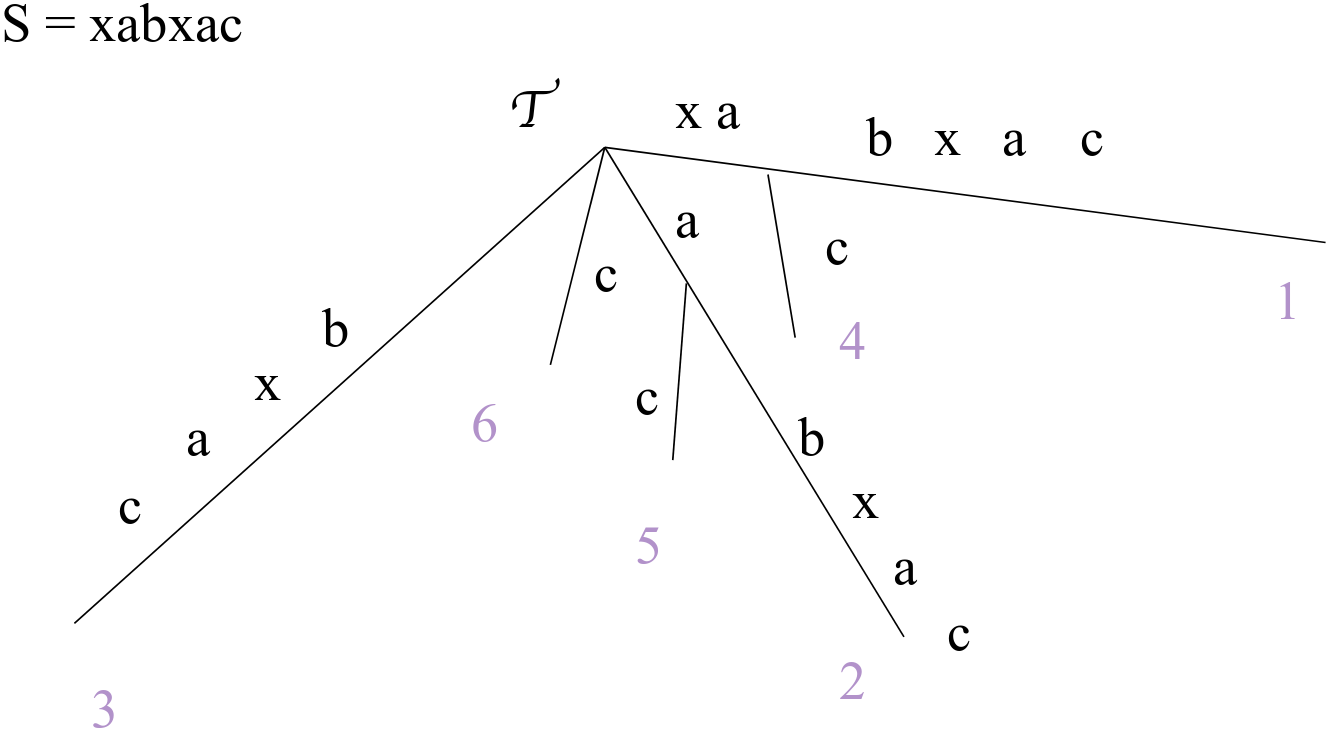
\includegraphics[width=0.9\textwidth]{img/suffix_tree.png}
		\caption{Example of suffix tree.}
		\label{f1}
	\end{minipage}
	\hspace{0.1cm}
	\begin{minipage}[t]{0.5\linewidth} 
		\centering
		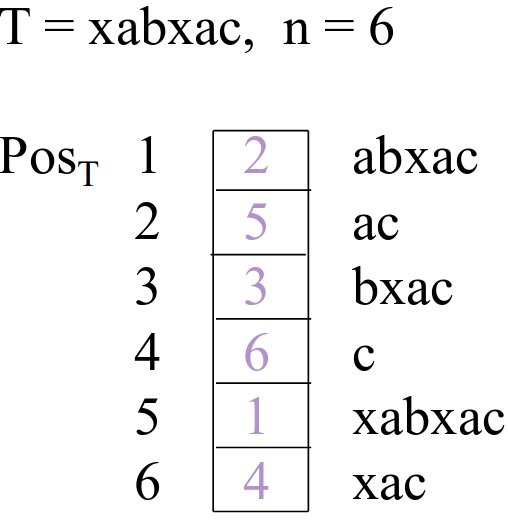
\includegraphics[width=0.5\textwidth]{img/suffix_array.png}
		\caption{Associated Suffix Array.}
		\label{f2}
	\end{minipage}        
\end{figure} 

Let us assume to have enough space to build the suffix tree for $T$ but not to save it permanently in memory. Then, Pos$_T$ can be obtained from the suffix tree for $T$ by \textit{traversing it "depth first in lexical order"}, with a time complexity $O(n)$. If in the suffix tree the sons of each node are already stored in lexical order, it is a simple depth-first traversing.

\subsection{Pattern matching with suffix array}
Once we have computed the suffix array the pattern matching algorithm is performed as follows:
\begin{itemize}
	\item if $P$ is contained in $T$, then all its occurrences are consecutive in Pos$_T$.
	$$\text{Ex:~P~=~xa}\quad \text{corresponds to Pos}_T[5]~=~1,\quad \text{Pos}_T~=~4$$
	\item In order to find the occurrences of $P$ in $T$ performs a binary search in Pos$_T$ comparing $P$ with the corresponding suffix of $T$:
	\begin{enumerate}
		\item with a binary search one can find the \textbf{first} occurrence of $P$ in Pos$_T$,
		\item with another binary search one can find the \textbf{last} occurrence of $P$ in Pos$_T$.
	\end{enumerate}
\end{itemize}
Complexity of the search of all the occurrences of $P$ of size $m$: $O(m~log~n)$, the worst case depends on how many long prefixed of $P$ are in $T$. Considering random strings we can have $O(m~+~log~n)$.
\image{img/searchPatternSuffixArray.png}{Search for a pattern}{0.6}
\subsection{mlr accelerator}
Let us assume there are many long prefixed of $P$ in $T$. We can optimize the pattern matching with the \textbf{mlr (minimum left right)} accelerator.
\begin{itemize}
	\item $L,R$ indicate the bounds of the search interval (at the beginning $L= 1$, $R = n$);
	\item $\mathcal{L}$ = length of the max common prefix between Pos$_T[L]$ and $P$.
	\item $\mathcal{R}$ = length of the max common prefix between Pos$_T[R]$ and $P$.
	
	$$Ex:\qquad P = xa,~ L = 4,~ R = 6 \quad \rightarrow \mathcal{L} = 0, \mathcal{R} = 2$$
	\item at each iteration in the binary search we inspect $M = \lceil\frac{L+R}{2}\rceil$.
	\item it is useless to compare $P$ with the prefix corresponding to Pos$_T[M]$ in the first mlr = min($\mathcal{L}, \mathcal{R}$) symbols. Then the comparison can start at symbol $mlr~+~1$
\end{itemize}

The cost of maintaining mlr is small, but it avoids many useless comparisons, optimizing the overall time complexity. The worst case is still $O(m~log~n)$, meaning that the symbols in $P$ from $mlr+1$ to $max(\mathcal{L}, \mathcal{R})$ are compared more than once.
Our goal is to reach a complexity equal to $O(m+log~n)$ also in the worst case, meaning that we need to reduce the number of useless comparison and any symbol in $P$ should be examined only once or a constant number of times.

\subsection{Super Accelerators Lcp}
It is possible to get $O(m+log~n)$ by using the super accelerators \textbf{Lcp(L,M)} and \textbf{Lcm(M,R)} besides $\mathcal{L}$ and $\mathcal{R}$ (more efficient, but more complex in the logic).\\


\paragraph{Definition.} $Lcp(i,j) = $ length of the longest common prefix between Pos$_T[i]$ and Pos$_T[j]$.
$$Ex:\qquad Pos_T[5]~and~Pos_T[6] ~\rightarrow~Lcp(5,6)~=~|xa|~=~2$$
For all $(L,M,R)$ we use $Lcp(L,M)$ and $Lcp(M,R)$ as accelerators, and note that Lcp values are defined on the text only, not on the pattern. Hence, they can be pre-computed and then used for pattern matching.

\paragraph{How to use accelerators.}

\begin{enumerate}
	\item \textbf{Simples case}: if $\mathcal{L} = \mathcal{R}(= mlr)$, then $P$ is compared with Pos$_T[M]$ starting at $mlr+1$, as in the algorithm with mlr accelerator.
	
	\item \textbf{General case}: $\mathcal{L} \neq \mathcal{R}$\\
	Let us assume $\mathcal{L} > \mathcal{R}$, that is $max(\mathcal{L},\mathcal{R}) = \mathcal{L}$ and $mlr = \mathcal{R}$. We can easily deduce that the symmetric case is reached when $\mathcal{L} < \mathcal{R}$, that is $max(\mathcal{L},\mathcal{R}) = \mathcal{R}$ and $mlr = \mathcal{L}$.\\
	Then we have $3$ different subcases:
	\image{img/superAccelerators.png}{How to use super accelerators}{0.8}
\end{enumerate}

\textbf{Property:} using the Lcp values, the search algorithm does at most $O(m~+~log~n)$ comparisons and runs in that time. For the proof look to the slides (pag 126).
The idea is that all symbols of $P$ are examined with $O(m)$ comparisons, there are at most $O(log~n)$ redundant comparisons, since for each iteration at most perform one redundant comparison (the last mismatch of $P$) and there are at most $O(log~n)$ iterations. So in total we can have a time complexity equal to $O(m~+~log~n)$.

\subsection{How to compute Super Accelerators}
Given a text of length $n$, the $Lcp$ values need to be pre-computed before using them for pattern matching. The time complexity of this operation is $O(n)$. For example, consider $n= 2^k$ and let $B$ the binary tree corresponding to all possible search interval, so that is has $n(n-1)$ nodes:
\image{img/LR.png}{B binary tree with $n(n-1)$ nodes}{0.7}

\textbf{Property:} Let $\mathcal{T}$ be the suffix tree for $T$ and $\varphi$ be the set of internal nodes traversed from the Pos$_T[i]$ and the leaf Pos$_T[i+1]$ during the lexical depth-first traversal. Let $v$ be the node in $\varphi$ closest to be root and let $\gamma$ be its label (the associated string), then $Lcp(i, i+1) = |\gamma|$.

\image{img/lcp.png}{Lexically ordered suffix tree}{0.8}
The algorithm used to compute the $Lcp(i, i+1)$:
\begin{itemize}
	\item $Lcp(i, i+1)$ can be computed while building the suffix array;
	\item The suffix tree can be built by annotating each node with its string depth 
	\item Then, the values $Lcp(i, i+1)$ can be computed by a lexical depth-first traversal of the suffix tree, while building the suffix array $ \rightarrow ~ O(n)$
	\item Let $\mathcal{L}_1$ be the traversed leaf and $\mathcal{L}_2$ the next leaf, if it exists, let us indicate $Lcp(\mathcal{L}_1,\mathcal{L}_2)$ with $Lcp(\mathcal{L}_1)$:
	\begin{itemize}
	\item if $\mathcal{L}_1$ has a right brother in the lexicographic order, then $Lcp(\mathcal{L}_1)$ is the string depth associated to their father node;
	\item If $\mathcal{L}_1$ is the last son, then $Lcp(\mathcal{L}_1)$ is the string depth of the closest predecessor of $\mathcal{L}_1$ which has further sons;
	\item if $\mathcal{L}_1$ is the last leaf, then $Lcp(\mathcal{L}_1) = 0$;
	\image{img/superAcceleratorProperty}{Property}{0.5}
	\end{itemize}

	\item In the binary tree $B$ (representing the search intervals), by associating the $Lcp(i,i+1)$ to the leaves, it is possible to compute the $Lcp(i,j)$, for $j~>~i+1$, by walking up from the leaves and setting the Lcp value at any node $v$ to the minimum of the Lcp values of its two children;
	\item Tree traversal requires visiting all nodes: $2n-1\quad \rightarrow ~ O(n)$.
\end{itemize}